\chapter{Continuation Theorems}\label{chap15} %lec 15

\section[Theorems about negative sequences,...]{Theorems about negative sequences, or sequences
  contained in a salient angle}\label{chap15:sec1} %Sec 1 

In\pageoriginale Lecture \ref{chap13}, we have seen how the principle of continuation can be
applied when the sequence $\Lambda$ consists of only negative
numbers. We had to suppose that the canonical product $C(w) = \prod
(1-\dfrac{w^2} {\lambda^2}) (\lambda \in \Lambda)$ satisfies
the condition that $\dfrac{|\log C' (\lambda)|} {\lambda}$ is bounded,
and that $\Lambda$ possesses a density or, at least, a, mean upper
density. Then, for a convenient $\Omega$, each $f \in 
\mathscr{H}_\Lambda (\Omega)$ can be ``continued'' in a certain
half-plane $x > x_o$. It is not a true continuation when $\Omega$ and
the half plane have no common points. Is it possible to consider the
function, defined in the half plane, as an analytic continuation of
$f$? This question will be solved by the use of result about minimum
moduls of $C(w)$, and a representation of $A_z (w)$ as a contour
integral. 

Suppose we fix arg $Z$ to satisfy the condition that $|\arg Z| <
\dfrac{\pi}{2} - \alpha, \alpha > 0$. Consider the contour $C$,
formed of the lines $[r\, e^{i (\pi - \alpha )}$, $r \,e^{i(\pi + \alpha )},
 0$ $\le r \le R ]$ and the circular are $[R e^{i (\pi + \theta)}
 |\theta| \le \alpha ]$, and taken in the positive direction. Let
$w$ be outside the angle made by this contour $C$. By Cauchy's
formula, we have the following equation: 
 \begin{figure}[H]
 \centerline{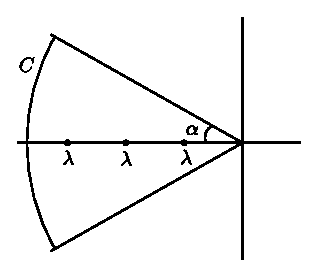
\includegraphics{vol15-figures/fig15-13.eps}}
 \end{figure}
$$
\frac{1}{2 \pi i} \int_C \frac{e^{w'Z} dw'}{C(w') (w-w')} =
\sum_{(\lambda \text{ inside } C)} \frac{e^{\lambda Z}}{C' (\lambda) (w-
 \lambda)} = A_C (w) 
$$
We\pageoriginale now apply Lemma \ref{chap14:lem1} to prove that the integral over the circular
arc of $C$ tends to zero when $R$ tends to infinity, along a
convenient sequence $\{ R_j\}$. We suppose that $\alpha$ is chosen so
that $|Z| \cos (\arg Z +\theta) < -2 \in < 0, \text{ for }
|\theta-\pi| < \alpha $. Then, by lemma \ref{chap14:lem1}, there exists a sequence
$R_j \nearrow \infty$ such that $|C (w')| > e^{- \in R_j}$
for $|w'| = R_j$. But $|e^{w'Z}| < e^{-2 \in R_j}$ and hence
the integral on the sector of radius $R_j $ tends to zero when $R_j
\to \infty$ 
\begin{align*}
 \text{Set}\hspace{2cm} A^+{(w)} & = \frac{1}{2 \pi i} \int_0^{\infty e^{i(\pi -
   \alpha )}} \frac{e^{w'Z} dw'} { C(w') (w-w')}; \hspace{2cm}\\ 
 A^+{(w)} & = \frac{1}{2 \pi i} \int_0^{\infty e^{i(\pi +
   \alpha)}} \frac{e^{w'Z} dw'} { C(w') (w-w')}. 
\end{align*}

If $A^+$ and $A^-$ exist, then $\lim\limits_{R_j \to \infty} A_C(w) =
A(w) = A^+ (w) - A^-(w)$. When $X \cos \alpha \pm Y \sin \alpha +
\frac{1}{R} \log |C(R e^{i \alpha })| > \in > 0 $ for large
values of $R$ and $Z = X+iY, A^+ (w)$ (\resp $A^- (w)$) defines a
function analytic outside the cone defined by the contour $C$ and
uniformly bounded in $Z$. 

When $w$ lies inside the cone defined by $C$, i,e., when $|\arg w -\pi|
< \alpha $ the same formula for $A(w)$ will hold if we adjoin to the
contour $C$ a small cut of the path of integration and a small circle
encircling $w$ on which $\int \dfrac{e^{w'Z} dw'} {C(w') (w-w')} = -2 \pi
i \frac{e^{wZ}} {C(w)}$. Such factors are uniformly bounded for $|w| =
R_j, |\arg w -\pi | < \alpha $. Thus we have $A(w)$ satisfying our
requirement of lecture 13; \S\ref{chap13:sec1}) it is uniformly bounded in $Z$
when $w$ varies outside the cone generated by $C$ or when $|w|= R_j,
|\arg w -\pi | < \alpha$; 2) it has polar part $ \sum\limits_\lambda
e^{\lambda z}/C' (\lambda) (w-\lambda)$, and 3) it is analytic
everywhere except at these poles) wherever $Z$ satisfies the
following conditions: 
\begin{enumerate}[a)]
\item for\pageoriginale a sequence of values of $R_j \nearrow \infty$, and for
 $|\theta -\pi| \le \alpha $ we have $|Z|$ $ \cos (\arg Z+\theta) -
 \frac{1}{R_j} \log | C(R_j e^{i \theta})| < -\in < 0$; 
\item for large values of $R$, we have 
$$X \cos \alpha \pm Y \sin
 \alpha + \frac{1}{R} \log | C (Re^{i (\pi \pm \alpha )})| >
 \in > 0, (Z= X + i Y).$$ 
\end{enumerate}

We will be able to find the variability of $Z$ satisfying these
conditions by making some more assumptions on $\Lambda$. 
\medskip

\noindent\textbf{1. $\Lambda$ possesses a density}

By the lemma of Carlson, if $\theta \nequiv 0 (\mod \pi)$, we have
{\small$\lim \frac{\log |C (R e^{i \theta})|} {R} = \pi D |\sin
\theta|$}. Using this and lemma \ref{chap14:lem3}, we are led to consider only
condition a) to determine the variability of $Z$. Moreover, by the
continuation developed in Lecture \ref{chap13} for negative sequence we have
the following theorem: 
\begin{theorem*}
 Suppose $\Lambda$ is a sequence of negative numbers having a density
 $D$ and $\Omega$ an open set containing the segment $(-i \pi D, i
 \pi D)$. Then it is possible to continue every function $f
 \in \mathscr{H}_\Lambda (\Omega)$ to be analytic in the
 right half-plane $ x \ge 0$. Moreover for $|\arg Z | < \beta <
 \dfrac{\pi}{2}$ the continuation yields us a function which is
 bounded and uniformly approximated by linear combination of
 $e^{\lambda z}, \lambda \in \Lambda$. If $\Lambda$ has a
 finite index of condensation $\delta$, the continuation yields us a
 Dirichlet's series convergent for $x \ge \delta$ 
\end{theorem*}

The same statement holds for a sequence $\Lambda$ without density, if
we replace $D$ by $D_{max}$. For there exists $\Lambda' \supset
\Lambda, \Lambda'$ having a density, and density $\Lambda' = D_{max}
\Lambda$ (see Appendix $1$) 
\begin{coro*}
 The sum of a Dirichlet's series whose sequence of exponents
 possesses a maximum density $D_{max}$, admits at least one
 singularity on every segment of length larger then $2 \pi D_{max}$
 on its abscissa of holomorphy. 
\end{coro*}

\noindent \textbf{2. $\Lambda$ has a finite mean upper density
  $\bar{D}^.$}

In\pageoriginale this case, by lemma \ref{chap14:lem8}, $|C (r e^{i \theta})| > 1$ for $|\theta
\pm \dfrac{pi}{2}| <\dfrac{\pi}{4}$. So, we are obliged to take into
consideration both the conditions a) and b) to determine the
variability of $Z$. As before the continuation developed for this case
in Lecture \ref{chap13}, gives us a similar theorem for continuation of $f
\in \mathscr{H}_\Lambda (\Omega)$, where $\Omega$ is an open
set the containing the circle $|z| \le \pi \bar{D}^.$, into that
portion of the right half plane contained between the lines $\theta =
\pm \dfrac{\pi}{4}$. The index of condensation $\delta$ is replaced by
the constant $B$. 

\noindent \textbf{3. $\Lambda$ is contained in a salient angle} 

Suppose $\Lambda$ is a sequence contained in a salient angular region
around the negative real axis, i.e., $\Lambda$ consists of points
$\lambda$ of the form $r e^{i (\pi +\theta)}, |\theta| \le
\beta$. Then using $|C (w)|< (1 + \dfrac{|w|^2} {|\lambda|^2})$ and
$|C (u)| < \prod|1 - \dfrac{u^2 e^{2 i \beta}}{|\lambda|^2}\big|$ for
locating the conjugate diagram and using $|C (w)| > \prod|1 -
\dfrac{w^2 e^{2 i \beta}}{|\lambda_2|^2 i \beta}\big|$ If $\dfrac
  {\pi}{2} < \arg w < \pi - \beta$ for having the minorization of
  $|C (w)|$ we can prove similar theorems taking $\alpha> \beta$
 \begin{figure}[H]
 \centerline{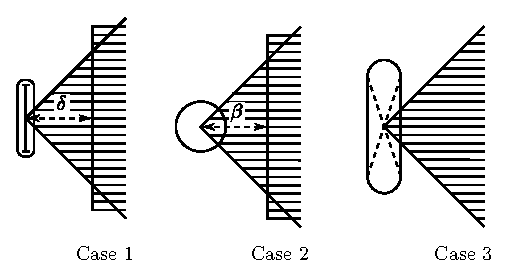
\includegraphics{vol15-figures/fig15-14.eps}}
 \end{figure}

\section{Theorems for symmetric sequences}\label{chap15:sec2}%Sec 2

First\pageoriginale let $\Lambda$ be a real symmetric sequence having a density
$D$. The canonical product $C(w) = \prod\limits_{\lambda \in \Lambda}
(1 - \dfrac{w^2}{\lambda^2})$ has for its conjugate diagram the
segment $(- i \pi D, i \pi D\lambda)^{\in \Lambda}$. Let $\Omega$ be
a domain containing this segment. The conjugate diagrams of $C(w) e^{w
 c}$ and $C(w) e^{-wc}, c > 0$, are two segments parallel to the
given segment and on either side of it. 

 \begin{figure}[H]
 \centerline{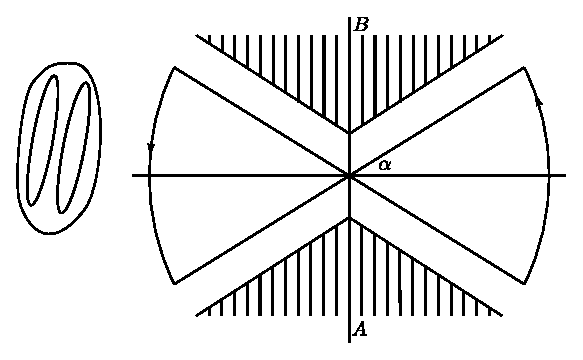
\includegraphics{vol15-figures/fig15-15.eps}}
 \end{figure}

For sufficiently small $c>0$, they are contained in $\Omega$. Now we
take $D(w) = C(w) Ch(cw) [ 2Ch(cw) = e^{wc} + e^{-wc}]$ in order that
we get a simultaneous majorization of $e^{w' Z}/ D(w') ~ (w-w')$ on
two circular arcs of the contour of integration situated
symmetrically. 

We take the contour $C$ consisting of the lines $re^{i \alpha}$ and
$re^{- i \alpha}, -R \le r \le R$ and circular arcs $Re^{i \theta} $
and $-Re^{i \theta}, - \alpha \le \theta \le \alpha$. Let $w$ be a
point with $\big | w - w' \big | > 1$ for any point $w'$ in the
interior of this contour. By Cauchy's theorem we have 
$$
A_C (w) = \frac{1}{2 \pi i} \int_C \frac{e^{w' Z} dw'}{D (w') (w-w')}
= \sum_{\lambda \text {inside} C} e^{\lambda Z}/D' (\lambda) (w-
\lambda). 
$$ 

Now, by Lemma \ref{chap14:lem1}, we have $\big | C(w) \big | > e^{- \in 
 R_j}$ on an infinity of circles of radii $1 R_j \nearrow \infty$ and
so taking into account the majorization 
$$
\big | e^{w' z }/ D (w') \big | < e^{r (R \big | \cos (\varphi +
 \theta) \big | + \in - C \big | \cos \theta \big | )} 
$$
where $Z = Re^{i \varphi}$, the integral on the circular arcs of $C$
vanish when $R_j \nearrow \infty$ if the following condition is
satisfied: 
\begin{equation}
 \begin{cases} R \cos (\varphi + \theta ) + \in - C \big |
 \cos \theta \big | < - \in ' \text for \big | \theta \big
 | \le \alpha, \big | \theta - \pi \big | \le \alpha. \tag{*} 
 \end{cases}
\end{equation}

If\pageoriginale the condition $(*)$ is realized we can proceed along the same line
of argument as on negative sequence by considering the positive and
negative parts of $\Lambda$ separately and we will have $A(w)$ bounded
and analytic inside the angles $A$ and $B$ as indicated in the figure, 
 \begin{figure}[H]
 \centerline{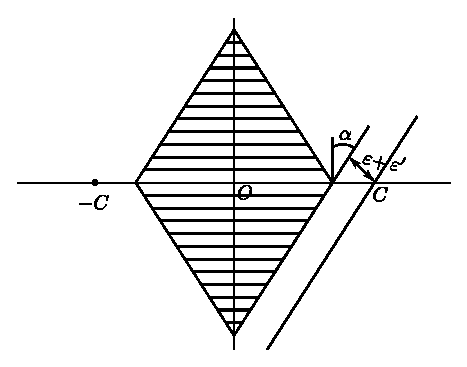
\includegraphics{vol15-figures/fig15-16.eps}}
 \end{figure}

In order to satisfy the condition $(*)$, the region of variability of
$Z$ for a given $\alpha$ is a rhombus with diagonals $(-c', c')$ and
$(- id, id)$ with $c' = d \tan \alpha= c - \dfrac{\in +
 \in '}{\cos \alpha}$. Since $\alpha$ is arbitrary, the
continuation is possible along a band around the imaginary axis. 

Such a problem of continuation was first considered by $A.F$. Leontiev
(Leontiev). Our method is different from that of Leontiev. The same
proof holds when $\Lambda$ is not necessarily real but accumulates
near the real axis, viz, arg $(\pm \lambda_n ) \to 0$ when $\lambda_n
\to \infty$. Thus we have the following theorem. 

\begin{theorem*}
 Let $\Lambda$ be a symmetric sequence accumulating near the real
 axis and possessing a density $D$. Let $\Omega$ be an open domain
 containing the segment $( - i \pi D, i \pi D) $. Then every function
 $f \in \mathscr{H}_\Lambda (\Omega)$ cam be analytically continued
 into a vertical band $\mathscr{B}$, (which may be degenerate into a
 half-plane or the whole plane) such that on each segment of length
 larger than $2 \pi D$ on the boundary of $\mathscr{B}$ there is at
 least one singularity of the function. 
\end{theorem*}

The\pageoriginale last part of the theorem results from the relation $f \in
\mathscr{H}_\Lambda (\Omega_\zeta)$ for every translate $\Omega_\zeta
$ of $\Omega$, such that $f$ is analytic along a chain of translates
joining $\Omega_\zeta$ to $\Omega$ (Lecture 12, \S 2). Moreover,
one can prove $f \in \mathscr{H}_\Omega (\mathscr{B})$ (Kahane 1, p. 98). 

Suppose now that $\Lambda$ is a symmetric sequence accumulating near
the real axis and having a mean upper density $\bar{D}^.$. The above
method can be applied, if we take $\alpha > \dfrac{\pi}{2}$, by using
lemma \ref{chap14:lem8} instead of lemma \ref{chap14:lem7}, Lecture
\ref{chap14}. This leads to the
following result. 

\begin{theorem*} %the 
 Suppose $\Lambda$ is symmetric, accumulates near the real axis, and
 possesses a mean upper density $\bar{D}^.t$. Take as $\Omega$ an
 open set containing the disc $| z | \le \pi \bar{D}^.$, and let
 $\Omega_c$ and $\Omega_{-c}$ be its translates by $c$ and $-c$,
 $\big | \arg c \big | < \dfrac{\pi}{4}$. Then every $f \in
 \mathscr{H}_\Lambda (\Omega_c \cup \Omega_{-c})$ can be continued
 in a rectangle whose sides make angles $\dfrac{\pi}{4}
 \pmod{\dfrac{\pi}{2}}$ with the real axis, and having $c$ and $-c$ as
 vertices. 
\end{theorem*}

\begin{figure}[H]
 \centerline{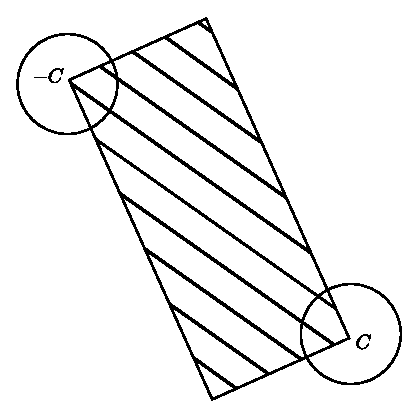
\includegraphics{vol15-figures/fig15-17.eps}}
\end{figure}
